\chapter{Introducción Específica} % Main chapter title

\label{Chapter2}
%
%%----------------------------------------------------------------------------------------
%%	SECTION 1
%%----------------------------------------------------------------------------------------
%La idea de esta sección es presentar el tema de modo que cualquier persona que no conoce el tema pueda entender de qué se trata y por qué es importante realizar este trabajo y cuál es su impacto.
%\label{sec:ejemplo}
En este capítulo se detallan las tareas que se realizaron, que contratiempos se tuvieron y cuales fueron los requerimientos.

\section{Objetivos y alcances}

\subsection*{Objetivos}
    El objetivo de este trabajo es desarrollar un software que permita controlar, monitorear y supervisar el proceso de fermentación del vino en las bodegas en forma automática. Para eso se utilizó la plataforma CIAA ya que está preparada especialmente para aplicaciones industriales.
\subsection*{Alcance}
  \begin{itemize}
      \item Sensar la temepratura de un tanque de fermentación de vinos.
      \item Controlar que la temperatura se mantenga dentro del rango correspondiente según el tipo de vino. 
      \item En caso de corte de energía notificar vía SMS a un celuar de contacto.
      \item Enviar mensajes de alerta vía SMS en caso de temperatura fuera de rango.
      \item Diseñar una página web para mostrar la información del sistema y realizar las configuraciones necesarias.
      \item Diseñar una placa básica para mostrar el funcionamiento del sistema.
  \end{itemize}

El proyecto no include:
  \begin{itemize}
    \item Estudio de los sensores y actuadores, se basara dicha información en los datos dados por el cliente. 
    \item Análisis del consumo eléctrico.
    \item Estudio del proceso de fermentación.
    \item Definición del rango de temperatura, esto será configurado por el cliente.
  \end{itemize}

  \section{Requerimientos}

Los requerimientos fueron consensuados con el responable de la Bodega Chico Zossi, para trabajar sobre un caso real y son los siguientes:

\begin{enumerate}[label*=\arabic*.]
  \item Medición de temperatura:
    \begin{enumerate}[label*=\arabic*.]
      \item Se requiere medir la temperatura de un tanque.
      \item Se tiene que poder definir un rango entre $7 a 30^oC$ con una apmlitud mínima de $1^oC$.
    \end{enumerate}
  \item Comunicación:
    \begin{enumerate}[label*=\arabic*.]
      \item Debe transmitir mensajes SMS notificando el estado y los cambios que se produzcan.
      \item Configuración de los parámetros requeridos de temperatura via web. 
    \end{enumerate}
  \item Funcionamiento del sistema embebido:
    \begin{enumerate}[label*=\arabic*.]
      \item El sistema deberá mantener la temperatura controlada a los parámetros configurados por el usuario. Para ello deberá hacer uso de actuadores.
      \item Deberá alertar si hay corte de energía mediante un SMS.
      \item Deberá mostrar el nivel de batería en porcentajes de 0 a 100\%  con una resolución mínima del 20\%. Y será mostrado en la página web.
  \end{enumerate}
\end{enumerate}


\section{Planificación del proyecto}
Para llevar a cabo el proyecto se desarrolló la planificación de tareas y se estimaron que tiempos debían emplearse para cada una de ellas.
Para esto se aplicó lo aprendido en la asignatura de Gestión de Proyectos y se estableció el diagrama de Grantt que se presenta en la figura \ref{fig:gantt}.  
A su vez se analizaron que tareas debían realizarse primero y cuales eran sus dependencias. De esta forma si se presentase alguna complicación se podría tener más claro cómo afectaría esto al proyecto.


\begin{landscape}
  \pagestyle{empty}
  \begin{figure}[htb]
      \centering
      %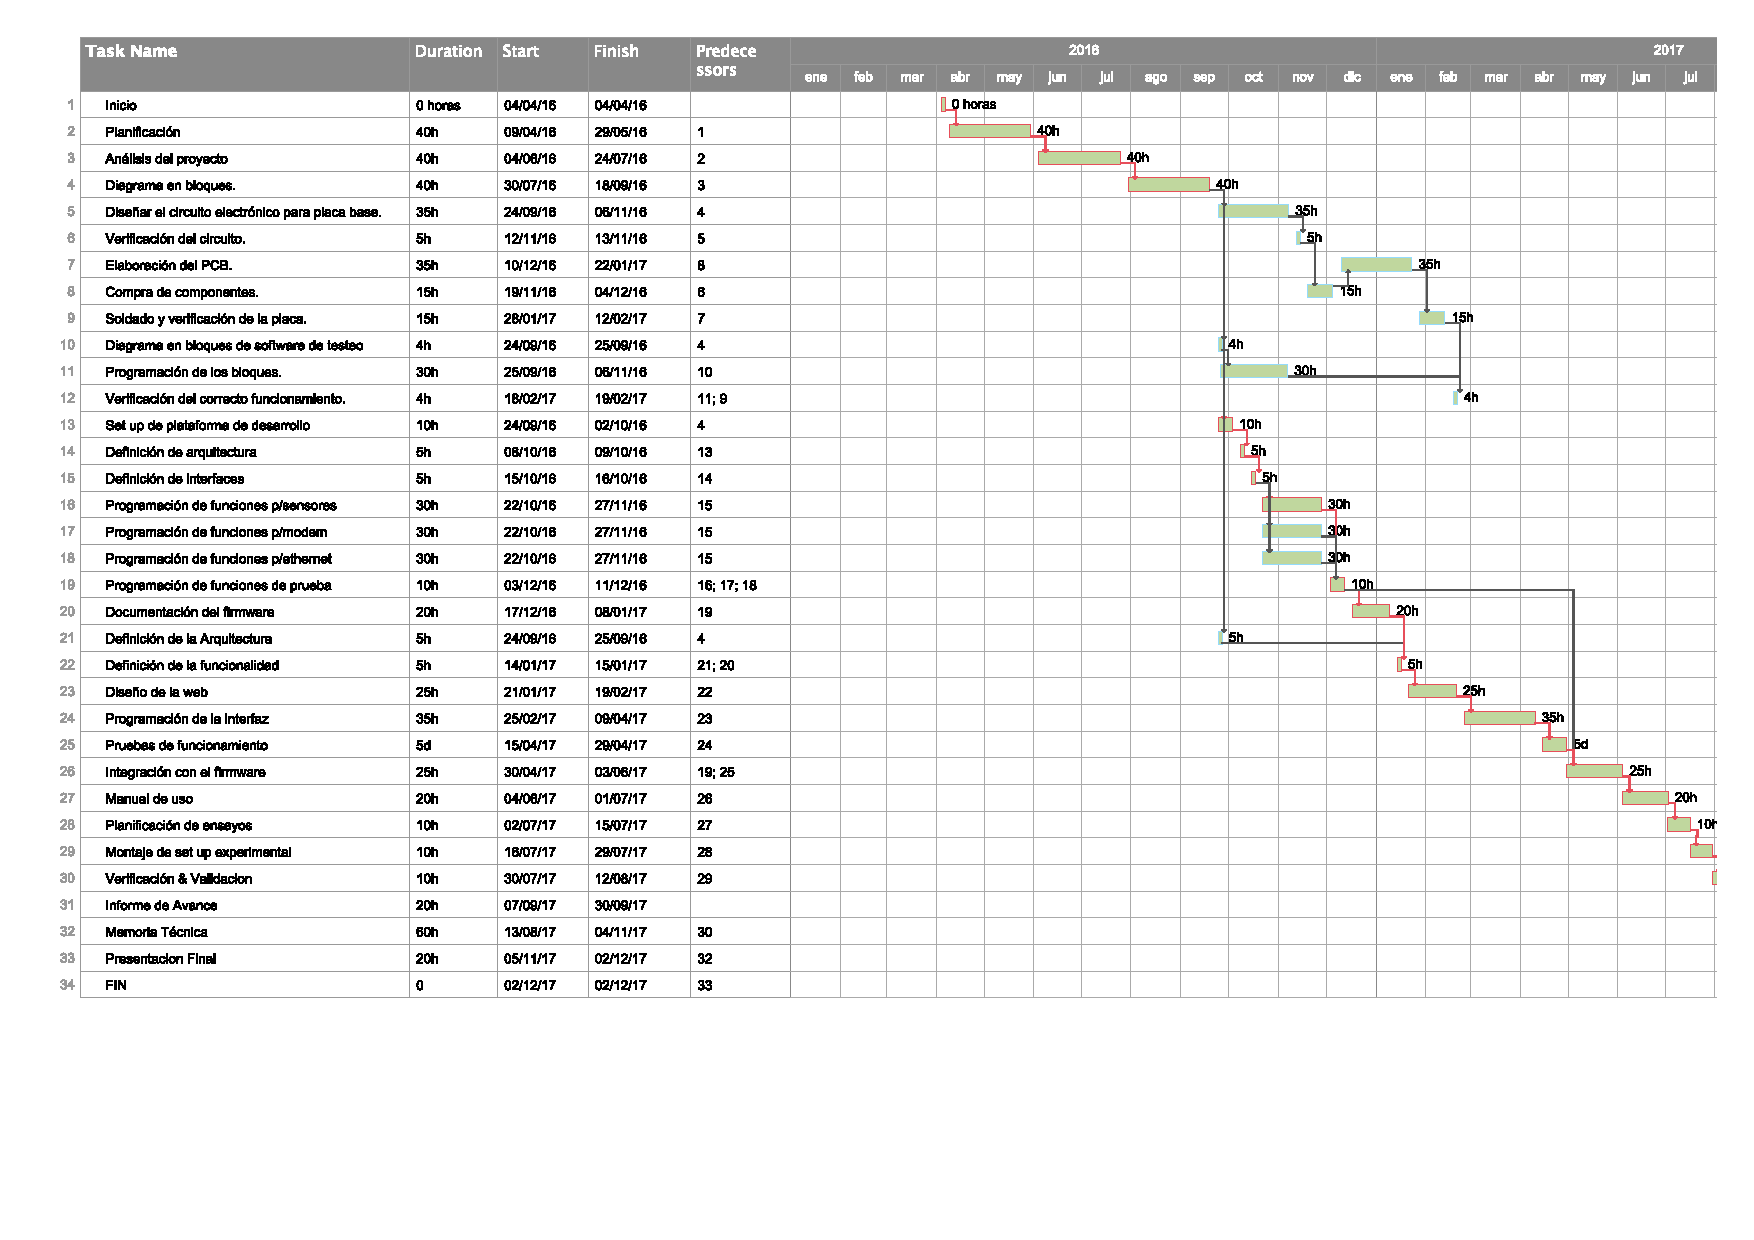
\includegraphics[page=1,clip, trim=0.5cm 4cm 16.3cm 0cm, width=1.00\textwidth]{./Figures/task_list.pdf}
          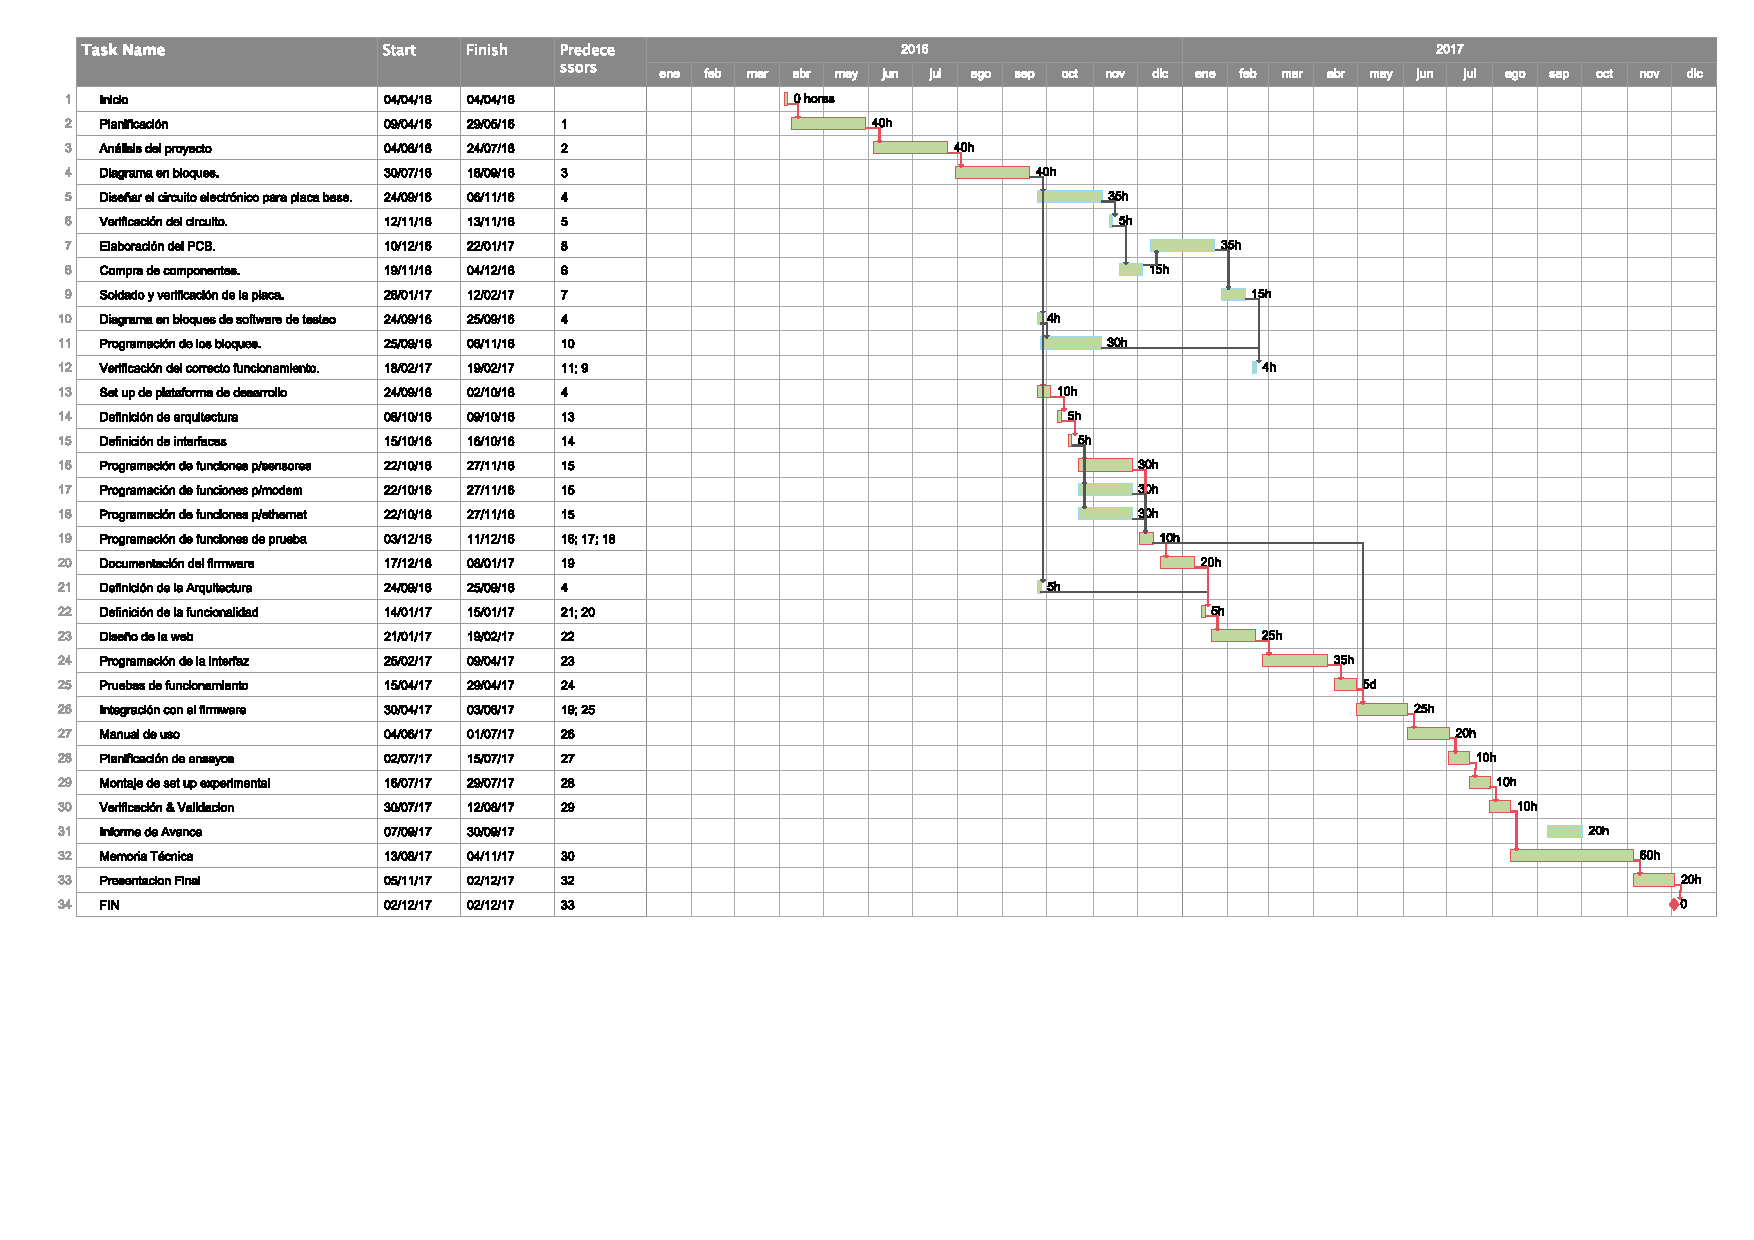
\includegraphics[page=1,clip, trim=0.5cm 5cm 0cm 0cm, width=1.70\textwidth]{./Figures/gantt.pdf}
      \caption{Listado de tareas, y plafinicacion de tiempos de la implementación.}
      \label{fig:gantt}
  \end{figure}
\end{landscape}


Al desarrollar el presente proyecto resultó que dada a la falta de experiencia en determinados temas se requirió más tiempo de lo planificado. En la tabla \ref{tab:update_task}, se aprecia el tiempo estimado, el tiempo realmente utilizado y cuales fueron las tareas que requirieron más tiempo.

\begin{table}[hp]
  \begin{tabular}{|c|c|c|c|c|}
    \hline
       &       & \multicolumn{2}{c|}{ Tiempo} & \%  \\ \cline{3-4}
    Nro& Tarea &       Estimado &  Real       & adicional \\
    \hline
    9 & Soldado y verificación de la placa & 15h & 24h & 60 \\
    18 & Programación de funciones p/ethernet & 30h & 50h & 66,7 \\
    23 & Programación de funciones p/ethernet & 25h & 35h & 40 \\
    \hline \hline
  \end{tabular}
  \caption{Comparación tiempo planificado vs real.}
  \label{tab:update_task}
\end{table}

Se observa una diferencia de 39 horas respecto a lo planificado. Siendo que para el desarrollo de todo el proyecto se habían estimado 617 horas podemos concluir que la estimación de los tiempos fue adecuada. 


